\documentclass[aspectratio=169,10pt]{beamer}

% Theme & Styling
\usetheme{Madrid}
\usecolortheme{whale}

% ITB Color Palette
\definecolor{ITBblue}{RGB}{0, 75, 141}
\definecolor{ITBgold}{RGB}{200, 150, 40}
\setbeamercolor{structure}{fg=ITBblue}
\setbeamercolor{title}{fg=white,bg=ITBblue}
\setbeamercolor{frametitle}{fg=white,bg=ITBblue}
\setbeamercolor{block title}{fg=white,bg=ITBblue}
\setbeamercolor{block body}{bg=ITBblue!8}

% Packages
\usepackage[utf8]{inputenc}
\usepackage{amsmath,amssymb}
\usepackage{graphicx}
\usepackage{hyperref}
\usepackage{multimedia}

\title[MA1101 Matematika I]{MA1101 Matematika I --- Bab 2: Turunan}
\subtitle{Subtopik 2.8: Laju yang Berkaitan (\textit{Related Rates})}
\author[FMIPA ITB]{Tim Pengajar MA1101}
\institute[ITB]{Fakultas Matematika dan Ilmu Pengetahuan Alam\\Institut Teknologi Bandung}
\date{Semester 1 Tahun Akademik 2026/2027}

\begin{document}

% -------------------------------------------------------------
% Slide 1: Judul
% -------------------------------------------------------------
\begin{frame}
    \titlepage
\end{frame}

% -------------------------------------------------------------
% Slide 2: Tantangan Sokratik (The Pique)
% -------------------------------------------------------------
\begin{frame}{Tantangan Awal: Tangga Meluncur di Dinding}
    \begin{columns}[T]
        \begin{column}{0.55\textwidth}
            \begin{block}{Eksperimen Pikir}
                Sebuah tangga dengan panjang $L = 5\text{ m}$ bersandar pada dinding tegak.
                Ujung atas tangga meluncur ke bawah dengan laju konstan:
                \[
                    \frac{dy}{dt} = -0.8\text{ m/detik}
                \]
            \end{block}

            \vspace{0.3cm}
            \begin{alertblock}{Pertanyaan Sokratik}
                Ketika tangga hampir rata dengan lantai ($y \to 0$):
                \begin{itemize}
                    \item Apakah ujung bawah melambat?
                    \item Bergerak dengan laju konstan?
                    \item Atau makin cepat melesat?
                \end{itemize}
            \end{alertblock}
        \end{column}

        \begin{column}{0.42\textwidth}
            \centering
            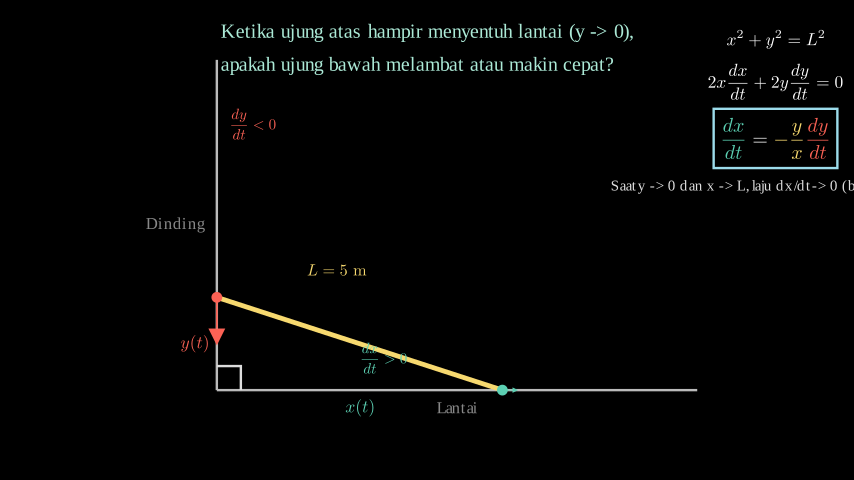
\includegraphics[width=\textwidth]{keyframe_tangga.png}\\
            \vspace{0.1cm}
            {\footnotesize \textit{Visualisasi Geometri Tangga Meluncur}}
        \end{column}
    \end{columns}
\end{frame}

% -------------------------------------------------------------
% Slide 3: Animasi Video Interaktif
% -------------------------------------------------------------
\begin{frame}{Simulasi Dinamis: Mengamati Laju Ujung Bawah}
    \centering
    % Embedded video untuk presenter (Pympress / PDFPC / Okular)
    \movie[width=9.6cm,height=5.4cm,poster,showcontrols=true]{%
        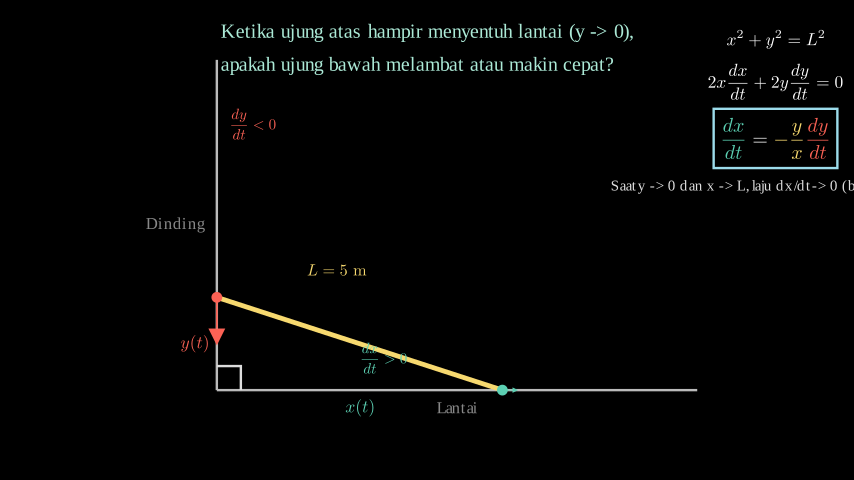
\includegraphics[height=0.55\textheight]{keyframe_tangga.png}%
    }{SlidingLadderScene.ogv}

    
    \vspace{0.2cm}
    \href{file:SlidingLadderScene.mp4}{%
        \beamergotobutton{\normalsize $\blacktriangleright$ Putar Video (\texttt{SlidingLadderScene.mp4})}%
    }
    
    \vspace{0.15cm}
    {\scriptsize \textit{Klik poster untuk memutar langsung di Pympress/Okular, atau klik tombol untuk membuka di MPV/VLC.}}
\end{frame}


% -------------------------------------------------------------
% Slide 4: Kristalisasi Matematis Formal
% -------------------------------------------------------------
\begin{frame}{Penurunan Matematis: Mengaitkan Dua Laju}
    \begin{columns}[T]
        \begin{column}{0.48\textwidth}
            \begin{block}{1. Hubungan Geometri (Pythagoras)}
                Pada setiap saat $t \ge 0$:
                \[
                    x^2(t) + y^2(t) = L^2
                \]
            \end{block}

            \begin{block}{2. Turunan Implisit terhadap $t$}
                Diferensialkan kedua ruas terhadap $t$:
                \[
                    \frac{d}{dt}[x^2 + y^2] = 0 \implies 2x \frac{dx}{dt} + 2y \frac{dy}{dt} = 0
                \]
            \end{block}
        \end{column}

        \begin{column}{0.48\textwidth}
            \begin{exampleblock}{3. Relasi Laju (\textit{Related Rates})}
                Menyelesaikan untuk laju horizontal $\frac{dx}{dt}$:
                \[
                    \mathbf{\frac{dx}{dt} = -\frac{y}{x} \frac{dy}{dt}}
                \]
            \end{exampleblock}

            \begin{alertblock}{4. Jawaban Teka-Teki Sokratik}
                Ketika tangga hampir rata di lantai ($y \to 0$ dan $x \to L$):
                \[
                    \frac{dx}{dt} \to -\frac{0}{L}\frac{dy}{dt} = 0
                \]
                Ujung bawah \textbf{melambat sesaat} sebelum berhenti!
            \end{alertblock}
        \end{column}
    \end{columns}
\end{frame}


% -------------------------------------------------------------
% Slide 5: Latihan Mandiri (Soal Ujian / Kuis)
% -------------------------------------------------------------
\begin{frame}{Latihan Terarah (Persiapan Kuis / UTS)}
    \begin{block}{Contoh Soal (Purcell / Stewart)}
        Sebuah tangga sepanjang $5\text{ meter}$ bersandar pada dinding tegak. 
        Jika ujung bawah ditarik menjauhi dinding dengan laju konstan $2\text{ m/detik}$,
        seberapa cepatkah ujung atas tangga meluncur ke bawah pada saat ujung bawah berjarak $3\text{ meter}$ dari dinding?
    \end{block}

    \pause
    \begin{columns}[T]
        \begin{column}{0.48\textwidth}
            \textbf{Langkah 1: Identifikasi Data}
            \begin{itemize}
                \item $L = 5\text{ m}$, $\frac{dx}{dt} = +2\text{ m/s}$.
                \item Saat $x = 3\text{ m} \implies y = \sqrt{5^2 - 3^2} = 4\text{ m}$.
            \end{itemize}
        \end{column}

        \begin{column}{0.48\textwidth}
            \textbf{Langkah 2: Substitusi ke Relasi Laju}
            \[
                \frac{dy}{dt} = -\frac{x}{y}\frac{dx}{dt} = -\frac{3}{4}(2) = -\mathbf{1.5\text{ m/detik}}
            \]
            \textit{Ujung atas meluncur ke bawah dengan laju $1.5\text{ m/detik}$.}
        \end{column}
    \end{columns}
\end{frame}

\end{document}
